\section{experiment Two Results} \label{results-2}
In this section, we first describe the participants' demographic in the second experiment. Then, we present descriptive statistics for the raw data. Lastly, we discuss results from our Bayesian analysis.

\subsection{Participant Demographics}
We collected 101 complete responses in the second experiment~\cite{illinoisdatabankIDB_1928463}. We removed 8 poor-quality responses where participants responded to the qualitative questions facetiously and put the same survey rating across all video elements. Among the remaining 93 participants, 55 of them identified as male and 38 as female. Around 80\% of the participants were White, 13\% were Black or African American, 5\% were Asian, and the remaining 2\% preferred not to disclose their racial information. Similar to experiment one, we aligned the participants' age and education level distribution to match that in the US 2018 census estimates~\cite{census2018}, as shown in \Cref{table:demo_exp2}.

\begin{table}
  \centering
  \caption{experiment two sample demographics statistics align closely with 2018 US census. } \label{table:demo_exp2}
  \sisetup{
    table-number-alignment = center, 
    table-figures-integer = 2, 
    table-figures-decimal = 2,
    round-mode = figures,
    round-precision = 3,
    detect-weight=true
  } \begin{tabularx}{0.5\textwidth}
    {@{}>{\raggedleft\arraybackslash}X>{\bfseries}SS@{}}
    \toprule
    Demographics & {Sample (\si{\percent})} & {Census (\si{\percent})} \\
    \midrule
    \textsc{\bfseries Education} & &\\
    No High School & 4.30 & 10.22  \\
    High School & 27.96 & 27.73  \\
    College  Associate & 31.18 & 33.09  \\
    Bachelor's Degree and above & 36.56 & 33.09  \\ 
    \textsc{\bfseries Age} & &\\
    18--24 & 9.68 & 13.65  \\
    25--39 & 39.78 & 30.74  \\
    40--54 & 27.96 & 28.32  \\
    55--69 & 22.58 & 27.29  \\
    \bottomrule\end{tabularx}
\end{table}

\subsection{Descriptive Statistics}

As shown in \Cref{fig:likert_exp2} and \Cref{fig:qv3_exp2}, on an aggregated level, participants expressed similar relative preferences across the five video elements in both Likert and QV. Audio quality ranked the highest in both cases, while motion smoothness and audio-video synchronization had the lowest ranks. While the aggregated preference were similar between Likert and QV, we will discuss their differences on an individual participant level in the next subsection. Similar to experiment one, a majority of the Likert response distributions skewed to the left; in contrast, QV response distributions approximated a Normal distribution. With a budget of 100 voice credits in QV, 57\% of the participants used at least 98\% of the budget and 82.8\% of them used over 90\% of the budget, suggesting that most participants actively made use of the majority of the budget.

\begin{figure}[htpb]
\centering
\begin{minipage}[b]{0.44\linewidth}
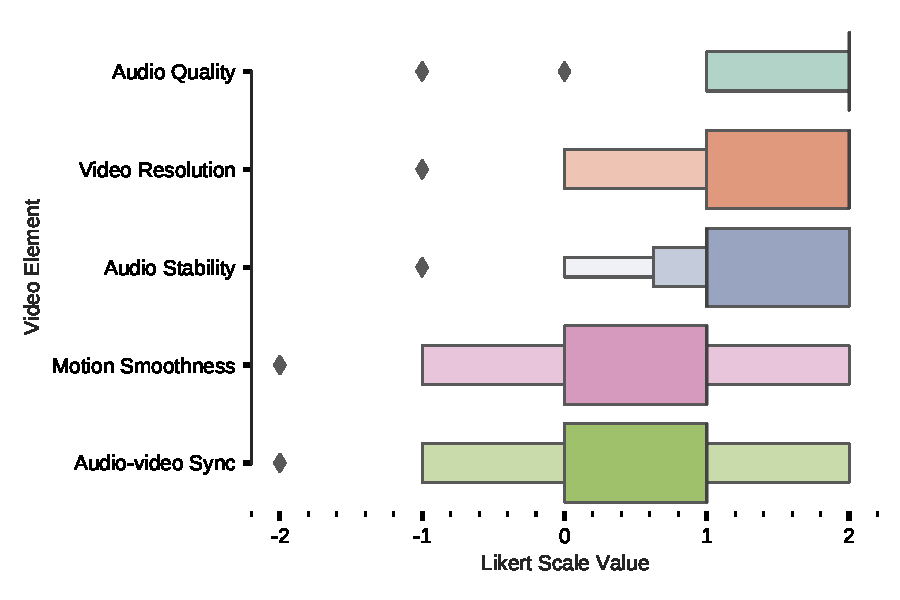
\includegraphics[width=\textwidth, keepaspectratio=true]{content/image/likert_distribution_per_element (1).pdf}
    \caption{
      Distribution of Likert scale survey responses per video elements in Boxen plot. 
      Each level from -2 to 2 corresponds to 
      ``Very unimportant'', ``Unimportant'', ``Neutral'', ``Important'', and ``Very important''.
      The distributions of different elements vary in their shapes, suggesting that participants showed their relative preferences even in the Likert group.
    }
    \Description[Distribution of Likert Responses per element for experiment two in Boxen plot]{Distribution of Likert Responses per element for experiment two in Boxen plot}
    \label{fig:likert_exp2}
\end{minipage}
\quad
\begin{minipage}[b]{0.52\linewidth}
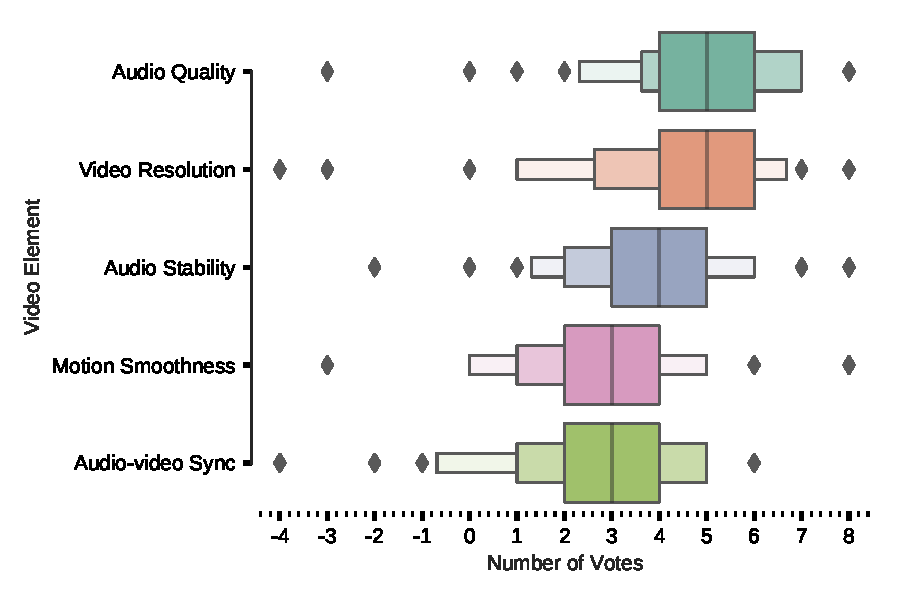
\includegraphics[width=0.9\textwidth, keepaspectratio=true]{content/image/qv_distribution_per_element.pdf}
    \caption{
      Distribution of QV responses per video element in QV in Boxen plots. The maximum possible number of votes on an element was 10 votes given 100 voice credits. Most distributions in all three QV set-ups follow a normal distribution. 
    }
    \Description[Distribution of QV Responses per element for experiment two]{Distribution of QV Responses per element for experiment two}
    \label{fig:qv3_exp2}
\end{minipage}
\end{figure}

\begin{figure}[ht]
    \centering
    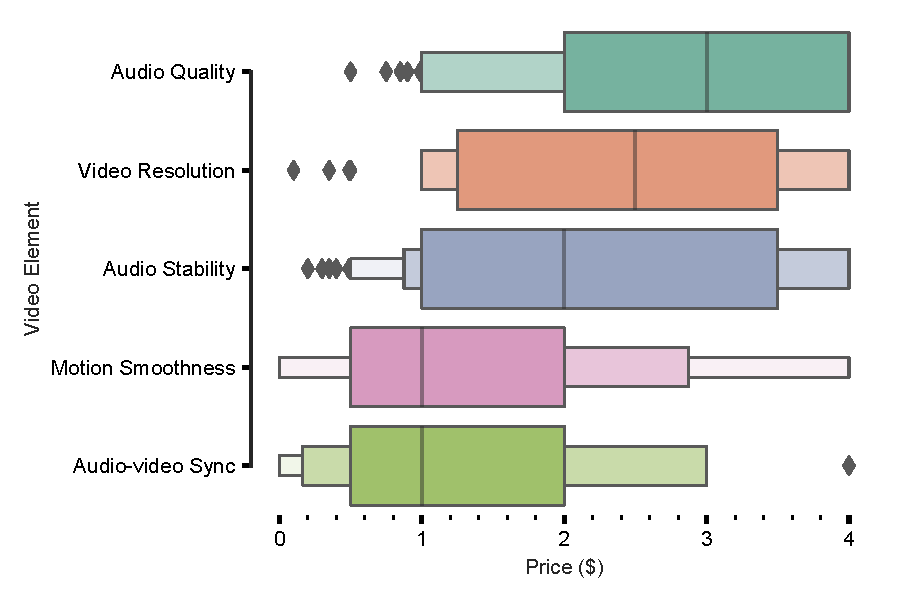
\includegraphics[width=0.5\textwidth, keepaspectratio=true]{content/image/price_distribution_per_element.pdf}
    \caption{
      Distribution of prices set by participants per video elements in Boxen plot. 
      Prices ranged from \$0 to \$4. Compared to the survey response distributions, elements with a higher rating of importance in surveys also had higher prices during product design.
    }
    \Description[Distribution of prices per element during the product design task in experiment two in Boxen plot]{Distribution of prices set for each element in experiment two in Boxen plot}
    \label{fig:price_exp2}
\end{figure}


Set prices for the five video elements exhibited similar patterns as the survey responses on an aggregated level (\Cref{fig:price_exp2}). Compared to the survey response distributions, elements with a higher average rating of importance in surveys also had higher average prices during product design. Since we instructed participants during price-setting that the buyer would be willing to pay more for the element that they value more, the alignment of preferences on an aggregated level between surveys and prices indicated that the participants kept our instruction in mind when they decided on the prices.


Similar to experiment one, we are interested in the degree of alignment between survey responses and prices set in an incentive-compatible scenario on an individual level. \Cref{fig:topic_covariate_exp2} visualizes the estimated correlation between normalized Likert or QV responses and normalized prices. All elements had a trend line with a positive slope, suggesting potential positive correlations. QV responses seemed to {\change{have}} a more positive slope with prices compared to Likert responses, indicating a possibly better alignment. Next, we present statistical support for this phenomenon.

\begin{figure}[htpb]
    \centering
    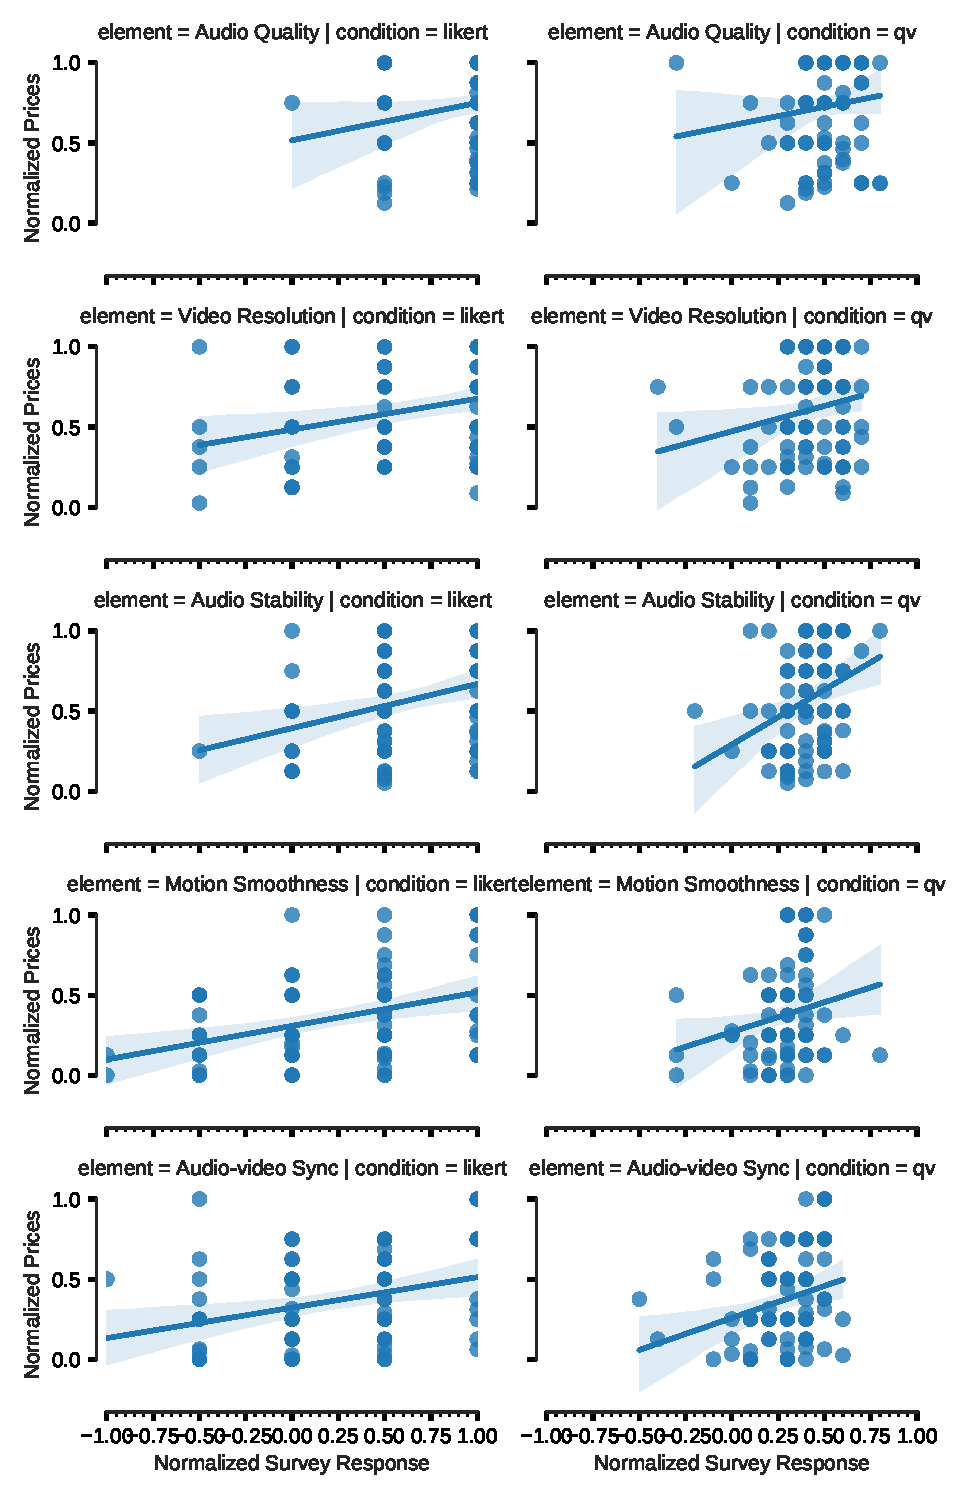
\includegraphics[width=0.6\textwidth, keepaspectratio=true]{content/image/correlation_per_element.pdf}
    \caption{
      Scatterplots showing the correlation between participants' normalized survey response and normalized prices for five video elements in the Likert survey and QV survey. Each row is one topic, and each column is one survey condition. \textbf{The main finding} is: all elements had a trend line with a positive slope, indicating potential positive correlations. QV responses seemed to {\change{have}} a more positive slope with prices compared to Likert responses, indicating a possibly better alignment.
    }
    \Description[Correlation scatterplots between normalized survey responses and normalized prices for experiment two]{
      Scatterplots showing the relationship between participants' normalized survey response and normalized prices for each of the five video elements in Likert and QV.
    }
    \label{fig:topic_covariate_exp2}
\end{figure}


\subsection{Bayesian Analysis Results}


\begin{figure}[htpb]
  \centering
  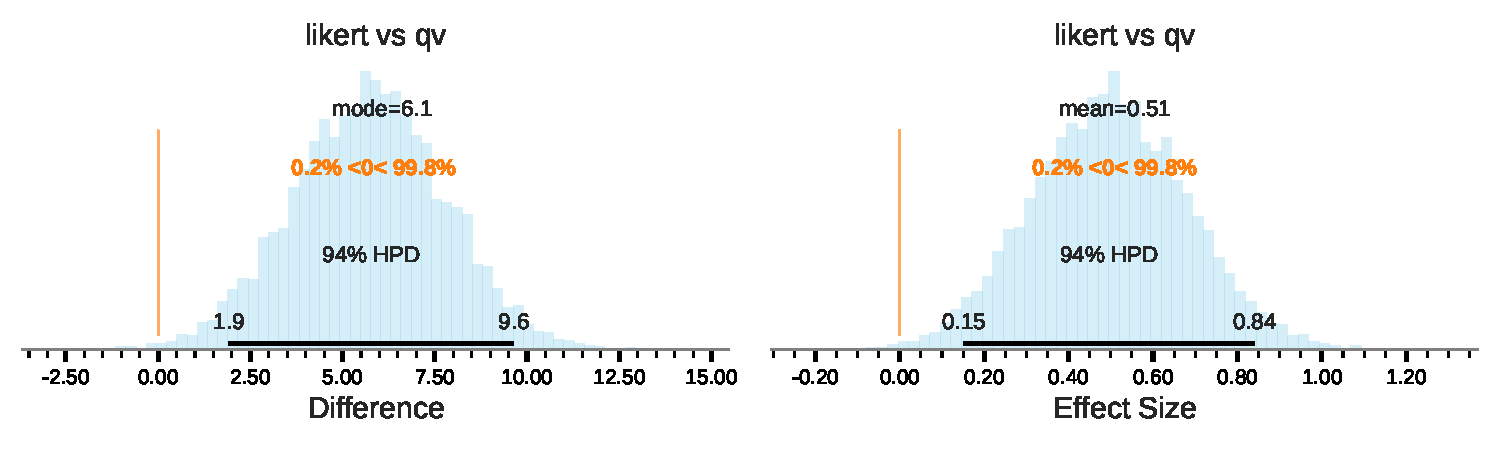
\includegraphics[trim= 0in 0in 0in 0in, clip, width=0.8\textwidth, keepaspectratio=true]{"content/image/Votes_Prices_StudentT_differences_and_effects.pdf"}
  \caption{
    The figure shows the contrasts distribution of the mean cosine similarity angles between the Likert group and QV group. The subgraph on the left shows the absolute difference while the one on the right is about the effect size. Since we are highlighting contrasts, each sub-figure shows an orange vertical line located at 0. \textbf{The main finding is:} survey responses from QV aligned significantly better with the price setting behavior than Likert scale responses with a medium effect size.
  }
  \Description[Contrasts distribution of the mean cosine similarity angles between Likert and QV for experiment two]{Contrasts distribution of the mean cosine similarity angles between Likert and QV for experiment two}
  \label{fig:contrast_exp2}
\end{figure}

Overall, our Bayesian analysis for experiment two showed that QV survey responses aligned significantly better with the price setting behaviors than Likert responses with a medium to high effect size (0.5--0.6). The first graph in the left column of~\Cref{fig:traceplot_exp2}, which contains traceplots for the MCMC estimations, shows that the distribution of the mean cosine similarity angle for QV (orange line) is to the left of that for Likert (blue line). Since a perfect alignment means a zero angle, QV had better alignment with the set prices relative to Likert. 

To confirm if the difference was statistical significant, we constructed the distribution of the absolute difference between the means and the distribution of the corresponding effect size (normalized difference), as shown in \Cref{fig:contrast_exp2}. In the subfigure on the left, the mode of the contrast is $6.1$, meaning that the cosine similarity angles in the Likert group were most frequently $6.1$ degrees larger than the angles in the QV group. Since the HPD of [$1.9$, $9.6$] lies outside a significant ROPE (Region of Practical Equivalence) of $0 \pm 1 \deg$, there was a significant difference between the alignment levels of the two survey methods. The medium to high effect size is significant based on the figure on the right, with a modal value of $0.51$ and a HPD interval of [$0.15$, $0.84$].


\begin{sidewaysfigure*}
  \centering
  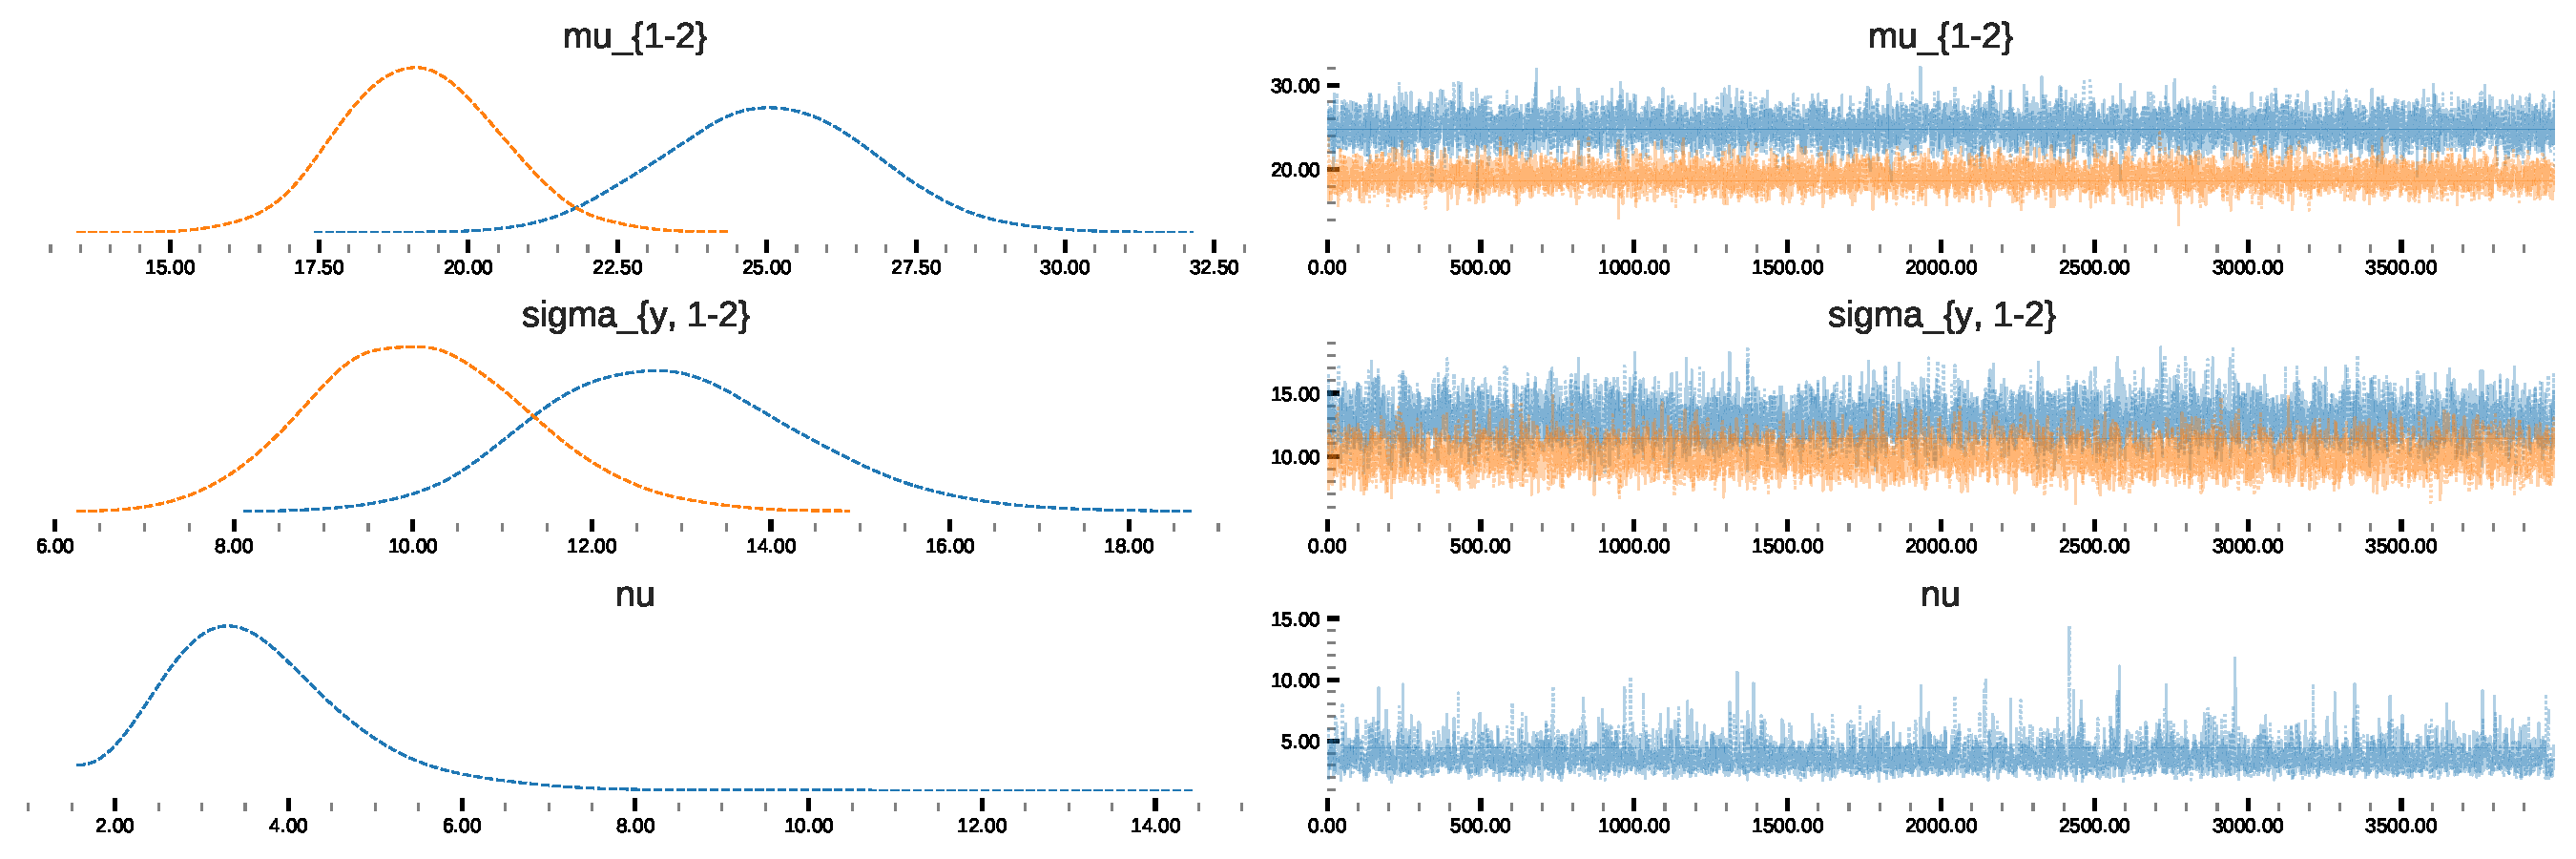
\includegraphics[trim= 0in 0in 0in 0in, clip, width=\textwidth, keepaspectratio=true]{content/image/StudentTIndep_traceplot.pdf}
  \caption{
    Traceplot showing the results of the MCMC estimation in experiment two. The left column is the posterior distributions for $\mu_{1-2}$, $\sigma_{1-2}$, and $\nu$ of the Student-t distribution. The right column shows the corresponding sampling traces. The color mappings are: orange -- QV, blue -- Likert. Distribution for $\mu_{1-2}$ of QV is to the left of Likert, meaning a better alignment with price setting behaviors. Note also, that the modal value for degrees of freedom $\nu \approx 3$, confirming our choice of the Student-t distribution instead of the Normal distribution, which usually requires $\nu \geq 30$. Furthermore, the Gelman-Rubin statistic $\hat{R}$ for all parameters was 1, indicating  convergence of the sampling MCMC chains.
  }
  \Description[Traceplot for the MCMC estimation in experiment two Bayesian model]{Traceplot for the MCMC estimation in experiment two Bayesian model}
  \label{fig:traceplot_exp2}
\end{sidewaysfigure*}